% Fundamental packages
\documentclass[11pt,a4paper,twoside]{book}
\usepackage[utf8]{inputenc}
\usepackage[american]{babel}
\usepackage{amsmath}
\usepackage{amsfonts}
\usepackage{amssymb}
\usepackage{graphicx}

% margins and general lay-out
%\usepackage[inner=3cm,outer=2cm,top=2.5cm,bottom=2.5cm]{geometry}
\usepackage[inner=2.5cm,outer=2.5cm,top=2.5cm,bottom=2.5cm]{geometry}
\pagestyle{plain}

% fonts (Helvetica) and typographical stuff 

\usepackage[T1]{fontenc}
\usepackage{lmodern} 
\usepackage{textcomp} 
\usepackage{pifont}
\usepackage{csquotes}
\usepackage{bm}

% Setting the font should be done after loading the typographic packages which tend to 
% set a new default font. The microtype package should however be loaded after the font ...
% using san serif helvetica clone
\usepackage{helvet}
\renewcommand{\familydefault}{\sfdefault}
% phv is another posibility.
% \renewcommand\rmdefault{phv}
\usepackage{microtype}

% additional packages
\usepackage{booktabs}
\usepackage{pdfpages}
\usepackage{hyperref}
\usepackage{float}
\usepackage{todonotes}
\usepackage{caption}
\usepackage{subcaption}
\usepackage{color}

% package to manage citations
\usepackage[backend=bibtex,style=authoryear-comp,sorting=nyt,isbn=false,url=false, natbib=true]{biblatex}
\addbibresource{references.bib}

% Kill the auto-indent
\setlength\parindent{0pt}

% test package
\usepackage{lipsum}

% Packages for list of symbols and list of abbreviations
%\usepackage[nonumberlist,acronym,toc,nomain]{glossaries}
%\makeglossaries
%\input{Glossaries/Abbreviations}

% new definitions
\newcommand{\expit}{\text{expit}}

\DeclareMathOperator*{\argmax}{arg\,max}

\DeclareMathOperator*{\argmin}{arg\,min}

% start of the document
\begin{document}

% include cover page + copyright statement + no pagenumbers
\pagenumbering{gobble}
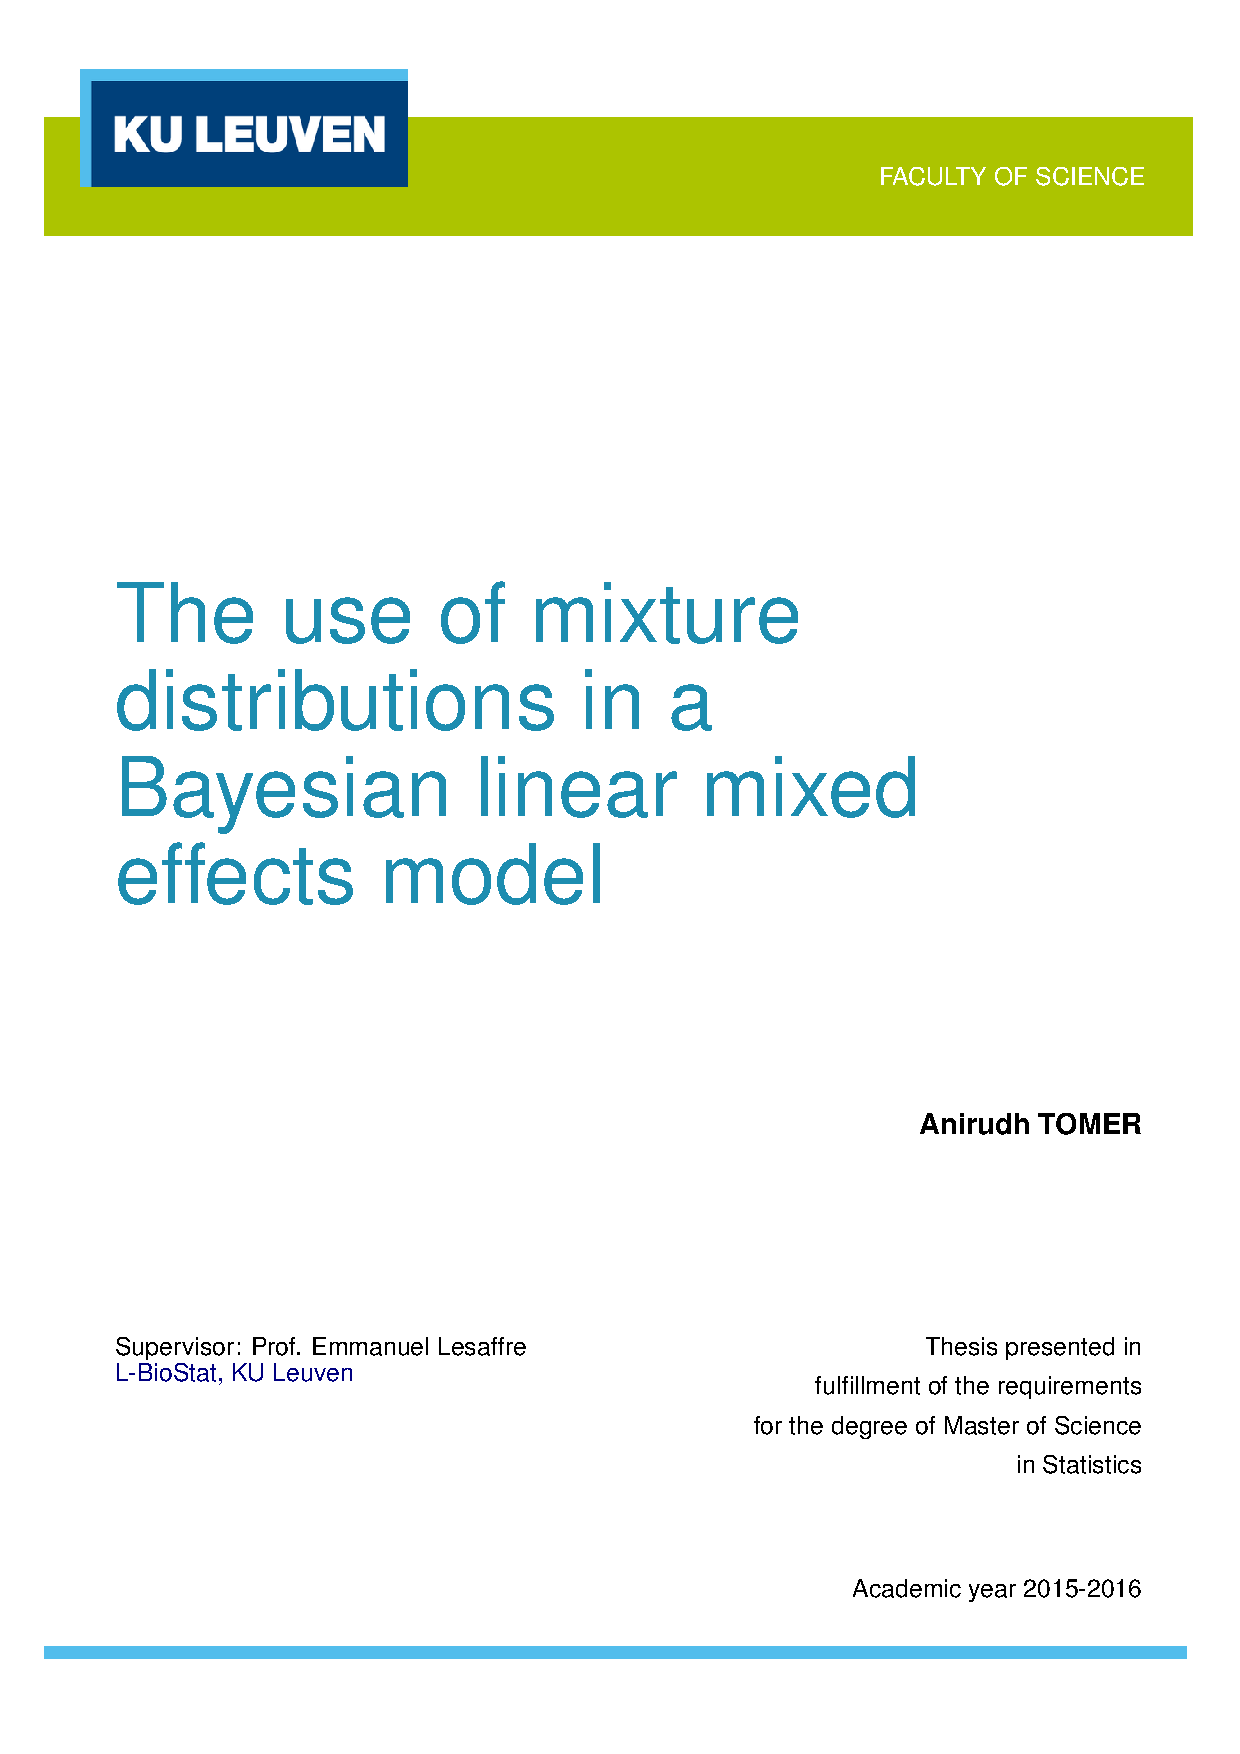
\includepdf[pages={1}]{coverpages/titlepage/titlepage.pdf}
%an empty page to make sure copyright gets printed on a new page
\clearpage \null \clearpage
\null
\vfill
\copyright~ Copyright by KU Leuven \\

Without written permission of the promotors and the authors it is forbidden to reproduce or adapt in any form or by any means any part of this publication. Requests for obtaining the right to reproduce or utilize parts of this publication should be addressed to KU Leuven, Faculteit Wetenschappen, Geel Huis, Kasteelpark Arenberg 11 bus 2100, 3001 Leuven (Heverlee), Telephone +32 16 32 14 01. \\

A written permission of the promotor is also required to use the methods, products, schematics and programs described in this work for industrial or commercial use, and for submitting this publication in scientific contests.
\cleardoublepage

% frontmatter + roman page numbers
\frontmatter

% !TEX root =  ../../thesis.tex

\chapter{Preface}
\label{ch : preface}

The following thesis work was conducted as part of the programme completion requirements of MSc. Statistics programme at KU Leuven. When I began working on this project, I had little idea that I would be able to go as far as I have been now. There were many significant obstacles on the way, such as analytical calculations of the various Deviance information criteria definitions, marginal likelihood, choice of posteerior predictive checks, implementating them in a software, Gibbs sampler idiosyncrasies and lack of computational power required for this work. However, at every step the work became more and more enticing. Looking backwards, I think it was one of the most interesting project I have done in recent times. Through and through, I enjoyed every bit of this project. The entire work for this thesis has been done using R and JAGS (Just Another Gibbs Sampler). The source code, results of simulations and an electronic draft of this thesis can be found at\\
\url{https://github.com/anirudhtomer/MScThesis}\\

In chapter 1 we present an introduction to mixture distribution and their central role in the formulation of the problem statement for this thesis. In Chapter 2 we present an introduction to the Bayesian paradigm as for the work of this thesis we use Bayesian methods. Futher in Chapter 3 we present the definition of a Bayesian heterogeneity model, and the issues with estimation of parameters in it. In Chapter 4 we present the formulae for various classes of Deviance information crieteria, marginal likelihood and posterior predictive checks that we used for model selection. Chapter 5 includes the results of the simulation study that was performed to check the efficacy of the aforemented Bayesian model selection methods. In chapter 6 we model the Blood donor data set \citep{nasserinejad_prevalence_2015} using a Bayesian heterogeneity model and use results from the simulation study to apply the right model selection criteria.\\

I am grateful to my supervisor Professor Dr. Emmanuel Lesaffre for keeping faith in my capabilities and for guiding me in the right direction. I enjoyed the fact that he never spoonfed me, yet was always available to discuss the difficult parts of the work at hand. He set very clear goals at the beginning of the year and continually monitored my progress thereafter. My interest in Bayesian statistics has grown by magnitudes under his supervision and I am looking forward to contribute more in this area. I would also like to extend my gratitude to Professor Geert Molenberghs and Professor Geert Verbeke for the captivating lectures on longitudinal data analysis. They introduced me to mixed models and empowered me with the tools of trade required to do the frequentist analysis of blood donor data set in this report. I am thankful to Kazem Nasserinejad from ErasmusMC for resolving many of my queries regarding the blood donor data set, and to Igor Milhoranca for providing the much needed inputs at crucial times. Lastly, I am grateful to my parents for the innumerable sacrifices they made to make sure I had as less obstacles as possible during my studies and I dedicate this work to them.\\

Anirudh Tomer\\
Leuven, Belgium\cleardoublepage
% !TEX root =  ../../thesis.tex

\chapter{Summary}
\label{ch : summary}

\todo[inline]{update the summary with the newest conclusions}

In this master thesis we fitted a finite mixture distribution for the random effects in a Bayesian linear mixed model. A mixture distribution for random effects allows to model the heterogeneity introduced by ignoring certain covariates in the mean structure of the model or to take into account the unknown non normal distriution for random effects. We then explored effectiveness of Bayesian model selection criteria (DIC, Bayes Factor, PPC) for choosing the number of component densities in the mixture distribution of random effects. Since mixture models are missing data models, we implemented various definitions of DIC as given by \citet{celeux_deviance_2006} for such models. We found that DIC 4 based on complete data likelihood was a fairly good selection criteria. However as the sample size decreased the discerning power of DIC also decreased. We then implemented Bayes Factor based on the approximation given by \citet{chib_marginal_1995} and found that it was not reliable for deciding on number of components required in the model. On the other hand, Posterior predictive checks were a very strong discerning method if indepdent inverse gamma priors were used for variance components, and uniform distribution for correlation, in the distribution of random effects. In regards to the choice of prior distribution for covariance parameters, we found that a Wishart prior for precision matrix(inverse of covariance matrix) overestimates the precision when within subject variance is greater than between subject variance. Thus, it could be a good idea to decrease scale of the intercept and the covariate corresponding to random slope, so that the corresponding variances increase in magnitude.
%\printglossary[type=\acronymtype,style=list,title={List of abbreviations}]
\cleardoublepage
\tableofcontents

% main matter (chapters + appendices
\mainmatter
% !TEX root =  ../../thesis.tex 

\chapter{Introduction}
\label{ch : introduction}

In this chapter we will first introduce the mixture distribution and then mention the challenges involved in estimation of parameters of a mixture distribution. We will also highlight the benefits of using a Bayesian approach for parameter estimation. Lastly we will present the goal of this master thesis, in which a mixture distribution plays the central role.

\section{Mixture distribution}
\label{sec : mixture_distribution}
A mixture distribution is a probability distribution of a random variable formed from a group of other random variables. The formation of a mixture distribution can be seen as a two step process, in which firstly a particular random variable is selected from a collection of random variables based on a certain probability of selection. In the second step a value is sampled for the selected random variable from its probability distribution. For e.g. the following random variable $Y$ has a mixture density formed from 3 normally distributed random variables.

$$Y \sim \dfrac{1}{6}N(-10,3) + \dfrac{1}{2}N(0,1) + \dfrac{1}{3}N(4,2)$$

\begin{figure}
	\centering
	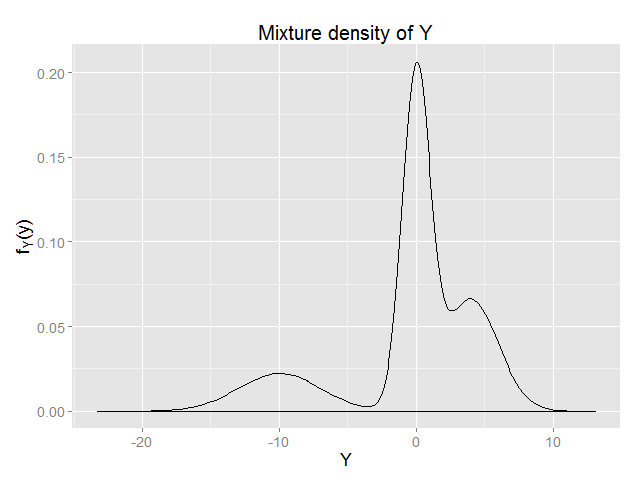
\includegraphics[scale=0.5]{mainmatter/chapter_1_introduction/mixture_density.png}
	\caption{Mixture density of $Y \sim \dfrac{1}{6}N(-10,3) + \dfrac{1}{2}N(0,1) + \dfrac{1}{3}N(4,2)$}
	\label{fig : mixture_density_1}
\end{figure}

Figure \ref{fig : mixture_density_1} shows the density function for $Y$. The density is trimodal with each mode corresponding to one of the components in the mixture. Mixtures like $Y$ which are formed from a finite sum of components are called finite mixtures. The components are also known as mixture components and their densities are called component densities. The constants multiplying the corresponding densities are called mixture weights. The mixture weights also represent the probability of selection of each component density. Each mixture weight should be positive and the sum of all mixture weights should be equal to 1. While in our example all the  mixture components were having the same parametric family i.e. Normal distribution, it is also possible to have mixture components from different parametric families. A mixture model where it is assumed that all data points are generated from a mixture of normally distributed component densities is called Gaussian mixture model (GMM). It is important to note that the idea of a mixture distribution is rather hypothetical, as in an example by \citet{titterington_statistical_1986} it was shown that a GMM of two components could be indistinguishable from a log-normal distribution.

\subsection{Formal definition for finite mixture distribution}
\label{subsec : formal_def_mixture_dist}
Given a finite set of $K$ probability density functions $p_1(y), p_2(y), \ldots, p_K(y)$ and weights $\eta_1, \eta_2, \ldots, \eta_K$, a random variable $Y$ is said to have a finite mixture distribution if

$$p(y) = \sum_{k=1}^{K} \eta_{k} p_{k}(y)$$

The vector of the weights $\boldsymbol{\eta} = (\eta_1, \eta_2, \ldots, \eta_K)^T$ is called the weight distribution. The $k^\text{th}$ weight $\eta_{k}$ corresponds to selection probability of the $k^\text{th}$ density while sampling for $Y$. It can only take values from the $K$ dimensional positive real coordinate space ${\mathbb{R}^{+}}^K$ with an additional constraint, $\sum_{k=1}^{K} \eta_{k} = 1$.\\

\subsection{Challenges}
\label{subsec : challenges_mixture_density}
The primary challenge while modeling a mixture density for a random variable is that the number of mixture components ($K$), weight distribution $\boldsymbol{\eta}$ and the corresponding parameters for component densities are rarely known in advance. Secondly, from a sample of $N$ observations $y_1, y_2, \ldots, y_N$ sampled from the mixture density $p(y)$ one may not know which observation belongs to which component density. Formally, an allocation vector $\boldsymbol{S} = (S_1, S_2, \ldots, S_N)^T$ represents the allocation of observations to mixture components. i.e. $S_i = k$ represents that $i^\text{th}$ observation belongs to $k^\text{th}$ component density. Estimating the allocation vector is in fact solving the clustering problem, albeit using parametric methods in our case.\\

While Maximum Likelihood based methods such as the EM algorithm could be used to deal with the above mentioned challenges, there are certain downsides to them. Firstly it is well known that 95\% confidence intervals of ML estimates are based on asymptotic normality of the estimators. Thus in case of small sample size, or small mixture weights the results will not be correct \citep[pg. 35]{fruhwirth-schnatter_finite_2013}. A Bayesian approach however is immune to these issues as the posterior distribution of parameters is allowed to be non-normal. Secondly, in case of univariate and multivariate GMM, the likelihood function

$$ p(\boldsymbol{y}|\boldsymbol{\mu}, \boldsymbol{\sigma^2}, \boldsymbol{\eta}) = \prod_{i=1}^{N} \sum_{k=1}^{K} f_N(y_i; \mu_k, \sigma^2_k) \eta_k$$

is unbounded and has many spurious nodes near the boundary of the parameter space for variance($\sigma^2_k$) of the components \citep{kiefer_consistency_1956,day_estimating_1969}. A Bayesian approach however, handles this problem elegantly using priors for parameters of the component densities. For e.g. \citet[pg. 176]{fruhwirth-schnatter_finite_2013} combined the likelihood with the prior $p(\mu_k, \sigma^2_k) \propto p(\sigma^2_k), \sigma^2_k\sim \text{Inv-Gamma}(1,4)$, and showed that it lead to a joint posterior density $p(\mu, \sigma^2 | \boldsymbol{y})$ of parameters in which $\sigma^2_k$ was bounded away from 0. Thus all the spurious nodes near the boundary of the parameter space for $\sigma^2_k$ were cut out, whereas they were apparent for the surface of the likelihood function.

\subsection{Applications of mixture distributions}
Mixture models have found usage in a variety of domains. Some of the examples are:
\begin{itemize}
\item Spike sorting of neural data: Both GMM and mixture of multivariate t-distributions have been used.\citep{lewicki_bayesian_1994,shoham_robust_2003}.
\item Speaker recognition as well as speech to text conversion algorithms have used mixture models \citep{simancas-acevedo_speaker_2001,xiang_efficient_2003,povey_subspace_2011}.
\item Image processing: GMM have been used to find features in an image, such as objects, boundaries etc. \citep{fu_color_2012}. For e.g. \citet{ming-hsuan_yang_gaussian_1998} have used GMM to model the distribution of skin color pixels. Many authors have also proposed using GMM for face recognition. i.e. as a biometric identification mechanism.
\item Finance: \citet{brigo_lognormal-mixture_2002} proposed to use a log-normal mixture distribution for pricing of financial assets.
\item Biology: Mixture models have found usage in genetics and cell biology.\citep{sim_evaluating_2012,gianola_mixture_2007} 
\end{itemize}

The example applications we cited involved usage of mixture models to adjust for a hidden attribute in the data which could not be collected or to approximate a density which is not of known form. However mixtures have also been used as supplementary methodology in various models, a list of which can be found in \citet[pg. 238]{fruhwirth-schnatter_finite_2013}. One such usage in linear mixed models has been proposed by \citet{verbeke_linear_1996} and it also forms the theme of this thesis.

\section{Goal of master thesis}
\label{sec : goal}
\citet*{verbeke_linear_1996} proposed to use a finite mixture distribution of normally distributed components for the prior distribution of random effects in a linear mixed effects model (LMM). This particular LMM is also known as Heterogeneity model. For the scope of this thesis our focus will be on the Bayesian version of the linear mixed effects model(BLMM), where all parameters involved are assigned a probability distribution. Needless to say, the issues described in section \ref{subsec : challenges_mixture_density} are also applicable for the Bayesian heterogeneity model. The aim of this master thesis is to evaluate existing Bayesian approaches for model selection, namely Deviance Information Criterion (DIC) , marginal likelihood and posterior predictive checks(PPC) for selecting the right number of mixture components for the distribution of random effects. Since we will be working in the Bayesian framework, we will use MCMC methods instead of the frequentist point estimation methods. We will simulate data sets to check efficacy of each of the aforementioned model selection criteria and then use the most effective ones to decide the number of mixture components for the random effects distribution in Blood donor longitudinal data set \citep{nasserinejad_prevalence_2015}.
% !TEX root =  ../../thesis.tex 

\chapter{Bayesian paradigm}
\label{ch : bayesian_paradigm}

\section{The bayesian motivation: A toy example}
To explain the motivation behind the bayesian paradigm, we will use an informal approach via the following toy example. Suppose there are three people A,B and C of whom A and B each are captains of a cricket team and C is the refree who tosses the coin. Given the importance of the toss in this sport each side would like to win the toss. Let us assume that based on experiences of an old friend captain B gets to know that the referee purposefully attempts at getting a heads on the toss. However given the nature of this problem, it is hard to quantify this belief in a single real number. Instead a belief that there is a 70 to 90\% chance that the result will be a heads is more likely than a belief that there is exactly an 80\% chance for the same. One might also have a slightly vague belief that there is more than 50\% chance that the toss will result into a heads. \\

\begin{figure}
\centering
	\begin{subfigure}[b]{0.45\textwidth}
		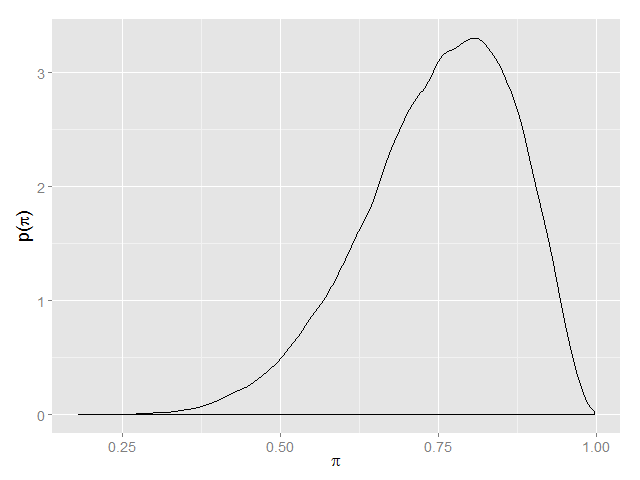
\includegraphics[width=\textwidth]{mainmatter/chapter_2_bayesian_paradigm/beta_prior.png}
        \caption{Prior $p(\pi)$: $\beta(9,3)$}
        \label{subfig : toy_problem_prior}
	\end{subfigure}
    	\begin{subfigure}[b]{0.45\textwidth}
		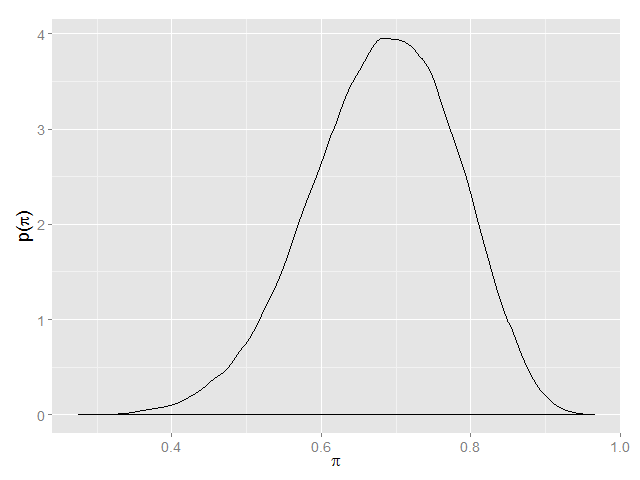
\includegraphics[width=\textwidth]{mainmatter/chapter_2_bayesian_paradigm/beta_posterior.png}
        \caption{Posterior $p(\pi|\boldsymbol{y})$: $\beta(15,7)$}
        \label{subfig : toy_problem_posterior}
	\end{subfigure}
\caption{Prior and posterior PDF for $\pi$; the probability of getting heads.}
\end{figure}

While subjective, these beliefs represent the prior probability distribution of a random variable in bayesian paradigm. In our toy problem the random variable is probability $\pi$ of getting a heads. For e.g. in figure \ref{subfig : toy_problem_prior} we can see one such prior distribution corresponding to the belief that the chance of getting a heads on toss is more than tails and it is more likely to be somewhere between 70 to 90\%. This is in contrast to the frequentist paradigm where parameters do not have a distribution but are rather constants. Also the point and interval estimation in frequentist paradigm do not take prior beliefs into account and rely completely on the data at hand. While a detailed discussion of Bayesian vs. Frequentist approaches can be found in \citet{lesaffre_bayesian_2012}, we will present a brief overview of Bayes theorem and its usage in bayesian parameter estimation.\\

\section{Bayes theorem}
\label{sec : bayes_theorem}
To understand the use of Bayes theorem in parameter estimation let us first look at one of the frequentist approach Maximum likelihood estimation to estimate the probability of getting heads ($\pi$). Suppose after 10 matches captain B observed that 6 times out 10 the toss resulted in heads. Assuming that conditions in each toss were such that the tosses were independent, then based on the likelihood function $L(\pi|\boldsymbol{y})$ the MLE of $\pi$ will be $\hat{\pi} = 0.6$. In contrast, the Bayes rule provides the framework to estimate the entire distribution of $\pi$ based on the data and the prior beliefs. The bayes rule for the continuous parameter $\pi$ is given by\\

\begin{equation}
\label{eq : bayes_rule}
p(\pi|\boldsymbol{y}) = \dfrac{L(\pi|\boldsymbol{y})p(\pi)}{p(\boldsymbol{y})} = \dfrac{L(\pi|\boldsymbol{y})p(\pi)}{\int_{0}^{1}L(\pi|\boldsymbol{y})p(\pi)d\pi}
\end{equation}

The result $p(\pi|\boldsymbol{y})$ is called the posterior distribution of the parameter based on which statistical inference about the parameter can be done. An intuitive way to get the motivation behind the bayes theorem is that the denominator can be seen as marginal probability of $\boldsymbol{y}$ based on the law of total probability. This is more evident in the categorical case though. In figure \ref{subfig : toy_problem_posterior} we can see the posterior PDF for the probability of getting heads that we obtained after applying Bayes rule. The mean value of this distribution is 0.7 which if you compare with the MLE of 0.6 you can see that bayesian posterior mean is influenced by the prior as well.\\
\todo[inline]{The intuition part is needed to be expanded upon, and shall I talk of CI at this moment???}

\section{Bayesian software}
We can see in equation \ref{eq : bayes_rule} that the computation of posterior involves solving the integral in the denominator. While the calculations are simple in certain cases, for e.g. in exponential family the choice of conjugate prior leads to a posterior belonging to the same family. However it also depends on the prior beliefs. For e.g. if the prior belief for $\pi$ in our toy example is that it is trimodal then we may have to use numerical approximation for calculation of the posterior. The most widely used algorithms for posterior approximation are Markov chain monte carlo (MCMC) techniques like Gibbs sampling, Slice sampling, Metropolis hastings and their variants etc.\\

The software tools we will use are from the BUGS family like JAGS or WinBUGS. While WinBUGS provides its own integrated development environment it definitely lacks the usability and visualization capabilities offered in R. JAGS on the other hand relies on third party tools completely for visualization and analysis of MCMC chains. There are R packages namely R2jags, R2WinBUGS which allow users to execute JAGS/WinBUGS code via R. For bayesian linear mixed models the R package blme will be used. For bayesian mixture models we will evaluate the R package bayesmix. The R package coda provides a rich array of functions to do analysis and diagnosis of MCMC chains.\\
% !TEX root =  ../../thesis.tex

\chapter{Bayesian linear mixed effects model}
\label{ch : blmm}

\section{Introduction to linear mixed model}
\label{sec : lmm}
A linear mixed effects model, also known as linear mixed model(LMM) is a statistical model for data which is hierarchical in structure. The specialty of the models is that apart from the fixed effects, they also model the correlation between the observations falling in the same group at a certain level in the hierarchy. The correlation is modeled with the help of random effects and the response is modeled as a linear function of both fixed and random effects.\\

There are many synonymous terminologies for data sets which are hierarchical in nature albeit with subtle nuances differentiating them. In this thesis our focus will be on Longitudinal data sets. A longitudinal data set is the one where multiple observations are collected from subjects at different points in time. For e.g. measurement of Hemoglobin of 20 patients with observations taken every month for a period of 24 months. Since the observations collected from a subject will be correlated a linear model will not be useful because of the restrictions it imposes on the covariance structure.\\

\todo[inline]{Should I mention that Laird and Ware proposed the model?}

\subsection{LMM definition}
\label{subsec : lmm_definition}
Following the notations from \citet{lesaffre_bayesian_2012}, the LMM for the observations of the $i^{th}$ subject among the $n$ subjects is given by\\

$$\boldsymbol{y_i} = \boldsymbol{X}_{i}\boldsymbol{\beta} + \boldsymbol{Z}_{i}\boldsymbol{b}_{i} + \boldsymbol{\varepsilon}_{i}$$\\

where $1 \le i \le n$,\\
$\boldsymbol{y}_i = {(y_{i1}, y_{i2}, \ldots, y_{im_i})}^T$ is a vector of observations for the $i^{th}$ subject taken at $m_i$ time points,\\
$\boldsymbol{X}_i = {(\boldsymbol{x}_{i1}^T, \boldsymbol{x}_{i2}^T, \ldots, \boldsymbol{x}_{im_i}^T)}^T$ is the $m_i \times (d+1)$ design matrix for the $i^{th}$ subject,\\
$\boldsymbol{\beta} = {(\beta_0, \beta_1, \ldots, \beta_d)}^T$ is a $(d+1) \times 1$ vector of fixed effects with $\beta_0$ being the intercept,\\
$\boldsymbol{Z}_i = {(\boldsymbol{z}_{i1}^T, \boldsymbol{z}_{i2}^T, \ldots, \boldsymbol{z}_{im_i}^T)}^T$ is the $m_i \times q$ design matrix of covariates varying for a subject at each observation,\\
$\boldsymbol{b}_i = {(b_{0i}, b_{1i}, \ldots, b_{(q-1)i})}^T$ is a $q \times 1$ vector of random effects with $b_{0i}$ being the random intercept. The random effects $\boldsymbol{b}_i \sim N_q(\boldsymbol{0}, G)$ with $G$ being the $q \times q$ covariance matrix,\\ 
$\boldsymbol{\varepsilon}_{i} = {(\varepsilon_{i1}, \varepsilon_{i2}, \ldots, \varepsilon_{im_i})}^T$ is a $m_i \times 1$ vector of measurement errors. The errors $\boldsymbol{\varepsilon}_{i} \sim N_{m_i}(\boldsymbol{0}, R_i)$ with $R_i$ being the $(m_i \times m_i)$ covariance matrix of errors,\\

The errors $\boldsymbol{\varepsilon}_{i}$ and the random effects $\boldsymbol{b_i}$ are assumed to be independent. $R_i$ is usually a diagonal matrix of the form $\sigma^2I_{m_i}$. While one might only model the correlation between the observations of a subject using random effects, it is also possible to model the serial correlation component. For this and an in depth coverage of LMM we refer the reader to \citet{verbeke_linear_2009}.\\

\section{Motivation for Bayesian linear mixed model}
\label{sec : blmm}
One of issues with the frequentist LMM is that while the parameters in matrices $G$ and $R_i$ are estimated using ML/REML only a point estimate is further used in estimation of fixed effects(see \cite[chap. 5]{verbeke_linear_2009}). Hence the uncertainty in estimation of random effects is ignored. Although frequentist inference approaches try to mitigate this issue by modifying the distributional assumptions of the test statistic \citep[pg. 56]{verbeke_linear_2009}, a bayesian approach considers the variability in parameter estimates in the first place. A similar problem occurs in the estimation of $\boldsymbol{b_i}$. The frequentist strategy is to use Empirical bayes estimates where the the posterior distribution of random effects uses point estimates of parameters in matrices $G$ and $R_i$. Thus the uncertainty in estimation is ignored. On the other hand the bayesian approach averages out over the entire posterior distribution of the hyperparameters to obtain the posterior $p(\boldsymbol{b_i}|\boldsymbol{y})$. In light of these reasons, in this thesis we will model our data using Bayesian linear mixed models.\\

The Bayesian linear mixed model or BLMM can be obtained by assigning a distribution to all the parameters involved in a LMM. This means that for the model presented in section \ref{subsec : lmm_definition} we will have a prior distribution for the following:
\begin{itemize}
\item $\sigma^2 \sim p(\sigma^2)$
\item $\boldsymbol{\beta} \sim p(\boldsymbol{\beta})$
\item $G \sim p(G)$
\end{itemize}

\section{Motivation for mixture of random effects}
As we saw above the random effects are assumed to be multivariate normally distributed. It could be too strong an assumption though in certain cases. A classical example of it are the longitudinal studies where at any time point we would like to categorize subjects in groups. For e.g. group with a high risk of having a certain disease in future vs. group with a low risk. While in retrospective studies it is quite easy as we know exactly which patients were diagnosed with the disease and which were not. However in a study where we would like to categorize patients into different groups well before diagnosis this could be difficult. Here is a toy example for it. Imagine that in longitudinal study we are measuring a response $Y$ which is an indicator of a disease. Assume that from a previous study it is known that patients which are in high risk group for the disease tend to have a higher response $Y$ during all times. Also assume that the trend of $Y$ over time remains the same for both groups otherwise. Figure \ref{fig : random_slope_dummy_data} shows individual profiles of subjects from a simulated dataset. Looking at this plot we can say that a random intercept component will be enough to model individual profiles. Since we will not be knowing which patient belongs to which group, this heterogeneity can be appropriately modeled by considering that the random intercept is a mixture of two normal components.\\

\begin{figure}
	\centering
	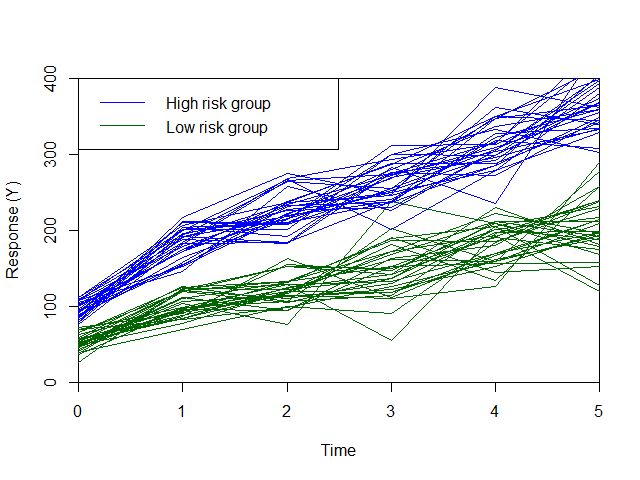
\includegraphics[scale=0.5]{mainmatter/chapter_3_blmm/random_slope_dummy_data.png}
	\caption{Individual profiles of 30 subjects from each group.}
	\label{fig : random_slope_dummy_data}
\end{figure}

In a LMM is quite common to use histogram of Empirical Bayes estimates of random effects to detect groups of individuals. However \citet{verbeke_linear_1996} have shown that if the prior is misspecified(for e.g. if in our example we use a single normal distribution), then it is possible that the histogram of estimates of random effects will be shrunk towards the prior distribution. This means that in our case we may not see a histogram with two distinct modes. The model where a mixture of Gaussian components were used to specify the random effects distribution is called a Heterogeneity model. Various applications of the heterogeneity model can be found in \citet[pg. 264]{fruhwirth-schnatter_finite_2013}.\\

\subsection{Mathematical notation}
Since the random effects are having a Gaussian mixture distribution we will use the following notation to express it mathematically.\\

$$\boldsymbol{b}_i \sim \sum_{k=1}^{K} \eta_k N_q(\boldsymbol{b}_k^C, G_k)$$\\
where $\boldsymbol{b}_k^C$ and $G_k$ are the mean vector and covariance matrices for the $k^{th}$ component in the mixture distribution respectively. The vector $\boldsymbol{\eta} = (\eta_1, \eta_2, \ldots, \eta_K)$ is the weight distribution for the component densities. Since we are following the bayesian paradigm, in addition to prior distribution for $\boldsymbol{\beta}$ and $\sigma^2$ we will now have prior for ($\boldsymbol{b}_1^C, \boldsymbol{b}_2^C, \ldots, \boldsymbol{b}_K^C, \boldsymbol{\eta}, G_1, G_2, \ldots, G_K$).

\section{Parametrization in BLMM}
The random effects $\boldsymbol{b}_i$ in a mixed model could be seen as random deviations from the fixed effects($\boldsymbol{\beta}$) with a mean $\boldsymbol{0}$. For a longitudinal data set, it means that the overall effect of a covariate like time for a subject should be the sum of both fixed and random effects. In this case matrices $\boldsymbol{X}$ and $\boldsymbol{Z}$ both share columns corresponding to the variable time. To enforce the mean $\boldsymbol{0}$ on the random effects in a mixture distribution the following condition should be satisfied.\\

$$E(\boldsymbol{b}_i | \boldsymbol{\phi}) = \sum_{k=1}^{K} \eta_k N_q(\boldsymbol{b}_k^C, G_k) = 0$$,\\
where $\boldsymbol{\phi}$ is the vector ($\boldsymbol{b}_1^C, \boldsymbol{b}_2^C, \ldots, \boldsymbol{b}_K^C, \boldsymbol{\eta}, G_1, G_2, \ldots, G_K$). This further means that $E(\boldsymbol{y}_i | \boldsymbol{\phi}) = \boldsymbol{X}_{i}\boldsymbol{\beta}$. This parametrization which was also used in the original paper on Heterogeneity model \citep{verbeke_linear_1996} is called noncentralized parametrization. The centralized parametrization assumes that the random effects are not deviations from the fixed effects and are centred around a non zero mean. The choice of parametrization has an effect on the rate of convergence while estimating parameters using MCMC. The non-centralized parametrization could be used when within subject heterogeneity is considerably smaller than the heterogeneity due to random effects. Otherwise a centralized parametrization is preferred. We refer the reader to \citet{fruhwirth-schnatter_bayesian_2004} for further details.

\section{Likelihood: Complete data vs Mixture}
The likelihood function in a mixture distribution depends on how much we know about the data. If we know both the data and the allocation vector $\boldsymbol{S}$ then the following likelihood function of parameters is called a complete data likelihood function.\\
$$p(\boldsymbol{y, S}|\boldsymbol{\nu}) = \prod_{i=1}^{N} \prod_{k=1}^{K} (p(\boldsymbol{y}_i | \boldsymbol{\theta}_k) \eta_k)^{I_{S_i=k}}$$\\
where $\boldsymbol{\nu} = (\boldsymbol{\theta}_1, \boldsymbol{\theta}_2, \ldots, \boldsymbol{\theta}_K, \boldsymbol{\eta})$ is a vector of weight distribution and parameters of component densities. It is possible to write this complete data likelihood function in $\perm{K}{K} = K!$ equivalent ways by permuting the order of components. Each order of components is called a Labeling scheme. Although this idea seems trivial we will see ahead that it creates a problem during estimation called label switching. While this likelihood function is valid conditional on knowing the allocation vector $\boldsymbol{S}$, the following likelihood function called Mixture likelihood function applies when we are not aware of the allocations.\\

$$p(\boldsymbol{y}|\boldsymbol{\nu}) = \prod_{i=1}^{N} (\sum_{k=1}^{K} p(\boldsymbol{y}_i | \boldsymbol{\theta}_k) \eta_k)$$\\

It is interesting to note that the mixture likelihood function is symmetrical and has $K!$ modes. We refer readers to \citet[pg. 45-46]{fruhwirth-schnatter_finite_2013} for the review of geometric presentation of this likelihood function.\\

\section{Mixture model identifiability: Label switching}
After running a MCMC procedure to estimate the posterior distributions of the parameters involved, we will be interested in knowing the parameters for the component densities. In most cases we will also be interested in classification of observation using allocation probabilities $P(S_i = k | \boldsymbol{y})$. Now let us imagine that we fitted exactly the true number of components ($K^{true}$ from which the mixture density was formed. At this point it is possible that the posterior densities of parameters do not reflect the true posterior distribution due to label switching.\\

To idea of label switching could be explained with this simple example. Suppose we have a mixture distribution $0.5N(5,1) + 0.5N(7,1)$of two components $C_1$ and $C_2$ and we sampled a few observations from it. The MCMC procedure we will estimate parameters using data augmentation. i.e. we begin with some random allocation vector $\boldsymbol{S}^0$ and estimate parameters using complete data likelihood. For MCMC labels $\mu_1$ and $\mu_2$ exist rather than  $\mu_{C1}$ and $\mu_{C2}$ and it does not associate labels with actual components. We begin with a vague joint prior for these parameters $p(\mu_1, \mu_2) = p(\mu_1)*p(\mu_2) = p(\mu_1)*p(\mu_1) = p(\mu_2)*p(\mu_2)$.\\

Assume that the allocation vector we began with assigns all observations from component $C_1$ to label 1 and all observations from component $C_2$ to label 2. Under such a scheme $(\mu_1,\mu_2) = (5,7)$ is likely. However if we take a conjugate of this allocation vector $(\mu_1,\mu_2) = (7,5)$ will also be accepted. This because we have a mixture likelihood function which is bimodal. Now let us imagine a scenario where because of our initial allocation vector, parameter estimates are $(\mu_1, \mu_2) = (5.5,6.5)$. So far it seems $\mu_1$ represents $\mu_{C1}$ and $\mu_2$ represents $\mu_{C2}$. Now we estimate allocation vector conditional on these estimates in MCMC. Supposing that an observation with value 6.5 originally from component $C_2$ gets allocated to component $C_1$ and similarly an observation with value 5.5 from component $C_1$ gets allocated to $C_2$. Unless we impose some constraint like $\mu_1 < \mu_2$, under the current situations even $(\mu_1,\mu_2) = (6.5, 5.5)$ could be sampled by MCMC. This because under the mixture likelihood it is also likely. However this scenario could've been unlikely if the true means were very far apart. In our scenario the issue is that posterior for $\mu_1$ will have a multiple modes. Not only that but if the sampler kept on arbitrarily switching between the two equivalent posterior regions then both regions will be partially explored. Thus any inference based on this posterior will be useless. \citet[pg. 82]{fruhwirth-schnatter_finite_2013} suggest to use a balanced label switching, which gives multimodal posterior albeit with a full exploration.\\

It is interesting that if our prior for the parameters was not vague, but exactly equal to the true distribution of parameters then label switching might not have happened. However the problem with a strong prior is that an incorrect strong prior could also inadvertently cause label switching or it might not allow a complete exploration of the posterior. Other techniques to stop label switching are imposing an identifiability constraint, which in our case was $\mu_1 < \mu_2$. However in higher dimensions it could become difficult to find a constraint which imposes a unique labeling scheme. For more details we refer the reader to \citet{stephens_dealing_2000}.\\

\section{Mixture model identifiability: Equal or empty components}
A mixture model will also be unidentified if we have an empty component or two components with the same parameters. Suppose the true number of components is $K^{true}$ and we fit $K = K^{true} + 1$ components. In the MCMC sampler suppose one of the components is assigned any observation. Thus the posterior for the parameters will remain the same as the prior. Assuming that the prior for weight distribution $\boldsymbol{\eta}$was a Dirichlet prior $\mathcal{D}(0.5, 0.5, \ldots, 0.5)$, then we will have a posterior for $\boldsymbol{\eta}$ such that the $K^{th}$ component will always have an almost 0 weight in the mixture distribution. This means that at the end of MCMC sampling the component density's posterior will be same as its prior and no observations will be allocated to the component. In such cases the true number of components could be estimated by the count of components with non zero number of allocations. However this situation could be avoided with a stronger prior on the weight distribution which forces the posterior distribution of $\boldsymbol{\eta}$ to be such that no components are empty at the end of MCMC sampling. Identification of number of components in such case is explained in the next section.\\

\textcolor{red}{Gosh! I should explain it in terms of pulling away the posterior eta from the boundary where components of eta are linearly dependent.}. 

\todo[inline]{Should I also discuss the choice of prior?}

\section{Choosing the right number of mixture components}
In most cases we do not know the right number of mixture components in advance unless we have some expert knowledge available or we know them from a previous/similar study. As part of this thesis we will compare many of the existing methods for finding the right number of mixture components.\\

\subsection{Information criteria based methods}
Information criteria are used to select models with parimony and good predictive power. Some of information criteria proposed in the literature are AIC proposed by Akaike, BIC (a minor modification of Schwarz's original criteria), DIC. While AIC and BIC are primarily used in frequentist statistics as they use point estimates of the parameters, DIC follows a more bayesian approach. Following are the definitions of the three criteria:\\

\begin{itemize}
\item $AIC = -2log(p(\boldsymbol{y}|\boldsymbol{\hat{\theta}})) + 2p$
\item $BIC = -2log(p(\boldsymbol{y}|\boldsymbol{\hat{\theta}})) + log(N)p$
\item $DIC = -2log(p(\boldsymbol{y}|\boldsymbol{\bar{\theta}})) + 2p_{DIC}$\\
where $\boldsymbol{\bar{\theta}} = E(\boldsymbol{\theta}_{post}|\boldsymbol{y})$,\\
$p_{DIC} = -2(E(log(p(\boldsymbol{y}|\boldsymbol{\theta}_{post}))) - log(p(\boldsymbol{y}|\boldsymbol{\bar{\theta}})))$ is the penalty for model complexity.
\end{itemize}

It is interesting to mention that the hierarchical nature of the mixture model implies a marginal model as well, which can be found by integrating out the random effects. \citet{verbeke_linear_1996} in their paper on heterogeneity model estimate the fixed effects and all covariance components using this marginal model. In our case y has a marginal model given by:\\

$$\boldsymbol{y_i} \sim \sum_{k=1}^{K} \eta_k N(\boldsymbol{X}_{i}\boldsymbol{\beta} + \boldsymbol{Z}_{i}\boldsymbol{b}_k^C,\boldsymbol{Z}_{i}G_{\boldsymbol{S}_i}\boldsymbol{Z}_{i}^T + R_i)$$\\

If our likelihood function is based on the marginal model then DIC could be used to select models which have good predictive power for an observation which is not necessarily from a subject who is in the current study. The total number of terms which will be penalized by AIC is equal to $dim(\boldsymbol{\eta}) + dim(\boldsymbol{\beta}) + dim(\boldsymbol{b}_{1}^C) + \ldots + dim(\boldsymbol{b}_{K}^C) + dim(G_1) + \ldots + dim(G_K) + 1(for \sigma^2)$, where dim is the total number of elements in the vector or matrix. On the other hand if we stick to the hierarchical interpretation, then DIC could be used to select models which have good predictive power for an observation which has to be from the current set of subjects. The total number of terms which will be penalized by AIC is equal to $dim(\boldsymbol{\beta}) + dim(\boldsymbol{b}_1) + \ldots + dim(\boldsymbol{b}_n) + 1(for \sigma^2)$. A model.

\subsection{Trans Dimensional Bayesian inference}
To compare a set of competing models $\mathcal{M}_1, \mathcal{M}_2, \ldots, \mathcal{M}_{K_{max}}$ each with their own set of parameters $\boldsymbol{\nu}_1, \boldsymbol{\nu}_2, \ldots, \boldsymbol{\nu}_{K_{max}}$ trans dimensional MCMC methods can be used. For e.g. Product space MCMC methods try to simultaneously sample the posterior probability $p(\mathcal{M}_{k}, \boldsymbol{\nu}_1, \boldsymbol{\nu}_2, \ldots, \boldsymbol{\nu}_{K_{max}}, \boldsymbol{y}$ for all $K_{max}$ models. The idea is that during each run a model indicator $\mathcal{M}$ which could follow for e.g. a multinomial distribution, is sampled. Suppose the model indicator is $M=2$ then all the parameters $\boldsymbol{\nu_{2}}$ are sampled whereas parameters for other models are kept what they were. The marginal posterior probability $p(\mathcal{M}_k|\boldsymbol{y}$ of the $k^{th}$ model is found by integrating out the parameters from the joint posterior. These could be further compared to select one of the K models.\\

\subsubsection{Marginal likelihood}
The ratio of marginal posterior could also be expressed as a Bayes Factor (assuming the prior probabilities for both models are equal) which is a ratio of Marginal likelihoods $\dfrac{p(\boldsymbol{y}|\mathcal{M}_i}{p(\boldsymbol{y}|\mathcal{M}_j}$ for the models. 
However \citet{johannes_berkhof_bayesian_2003} also suggest to use goodness of fit measures to be used along with Bayes factor. This because bayes factor is a relative measure. Relying on it completely could lead to selection of a model which is relatively better but overall does not provide a good fit.

\subsection{Posterior predictive checks}


\subsection{Other methods}
We will also explore other graphical methods or informal methods like method of moments in this thesis. For further reading on them we refer the reader to \citet[pg. 107-114]{fruhwirth-schnatter_finite_2013}
\chapter{Data set}
\label{ch:data_set}

\todo[inline]{Write something here}

\chapter{Analysis of data}
\label{ch:analysis_of_data}

\todo[inline]{Write something here}

\chapter{Conclusion}
\label{ch : conclusion}

\todo[inline]{Write something here}


% Appendices should go here
\appendix

% backmater => mainly references
\backmatter
\printbibliography
\cleardoublepage


\includepdf[pages={1}]{coverpages/backpage/backpage.pdf}
\end{document}
